%
%                       This is a basic LeTeX Template
%                       for the First Year PhD literature review 
\documentclass[a4paper,12pt]{article}
\usepackage{head,fullpage}     % Add local fullpage and head macros
\usepackage[pdftex]{graphicx}  % Add graphicx pachage with pdf flag (must use pdflatex)
\usepackage{datetime}

\newdateformat{monthyeardate}{%
  \monthname[\THEMONTH], \THEYEAR}
\parindent=0pt          %  Switch off indent of paragraphs 
\parskip=5pt            %  Put 5pt between each paragraph  
%
%                       This section generates a title page
%                       Edit only the sections indicated to put
%                       in the project title, your name, supervisor,
%                       project length in weeks and submission date
%
\begin{document}
\begin{minipage}[b]{110mm}
        {\Huge\bf School of Physics %\\and Astronomy
        \vspace*{17mm}}
\end{minipage}
\hfill
\begin{minipage}[t]{40mm}               
        \makebox[40mm]{
        
\includegraphics[width=40mm]{assets/tcd.logo.png}}
\end{minipage}
\par\noindent                                           % Centre Title, and name
\vspace*{2cm}
\begin{center}
        \Large\bf The Fast  Transient Sky\\
        \Large\bf Literature Review
\end{center}
\vspace*{1.5cm}
\begin{center}
        \bf Owen Johnson\\   
        \monthyeardate\today            % Submission Date
\end{center}
\vspace*{5mm}
%
%                       Insert your abstract HERE
%                       
\begin{abstract}
        The abstract is a short concise outline of your 
        project area, {\bf of no more than 100 words}.
\end{abstract}

\vspace*{1cm}

% \vspace*{3cm}
% Signature:\hspace*{8cm}Date:

\vfill
{\bf Supervisor:} Assoc. Prof. Evan Keane                % Change to suit
\newpage
%                                               Through page and setup 
%                                               fancy headings
\setcounter{page}{1}                            % Set page number to 1
\footruleheight{1pt}
\headruleheight{1pt}
\lfoot{\small School of Physics}
\lhead{Literature Review}
\rhead{ \thepage}
\cfoot{}
\rfoot{Date: 18-5-09}
%
\tableofcontents                                % Makes Table of Contents
\section{Background}

Outline the background of your subject area including the key initial
References \cite{jr:ashkin} and reference textbooks \cite{ob:bornwolf}. 
Also include some of the more
readable articles in popular science journals \cite{jr:dholakia},
and, where appropriate, standard textbooks \cite{ob:hechtoptics}.

The exact length of this section will depend on your subject area,
but will generally not exceed a page and will be aimed at the 
{\it general scientific reader}. 

\section{Review of Background Bibliography}

In this section detail the main supporting references
and articles \cite{jr:block} for your intended area of research
and, most importantly, your critical evaluation of their
relevance.  Also where your subject draws from multiple 
disciplines, do not forget to include key reference from
each discipline, even if they are relatively old \cite{jr:dammann}. 


This is the main part of your review and is the part that
will be of use to you when preparing for your thesis. Here try
and identify as many of the key references as possible, and enter then
into a {\tt BibTeX} file that you will use later. Remember that recording
the page number, titles and details of these 
key articles {\it now} will save you hours of
searching through {\em Web-of-Knowledge} the day before your
submit your thesis!

This part should be written in standard scientific language, 
aimed at the {\em experts in the field}. This is the main part of your first year report, and is 
expected to be 10 pages in length.

\section{Progress to Date}

In this section you should detail your progress to date. The length of this section
will depend on the type of research project you are undertaking.  

\section{Proposal}

In this section, detail, as far as you are currently able, 
your research plan for the second and third years of your PhD, 
drawing from the key references \cite{jr:block} that you have highlighted in your review section. 
Here, try and illustrate
your proposal, as in Figure~\ref{fig:prism} which is taken from the
same paper as the illustration references.
%
%                       Here is how to inserted a centered
%                       pdf file, this one is actually
%                       out of Maple, but it will work for other
%                       figures out of Xfig, Idraw and Xgraph
%
% \begin{figure}[htb]     %Insert a figure as soon as possible
%         \begin{center}
%           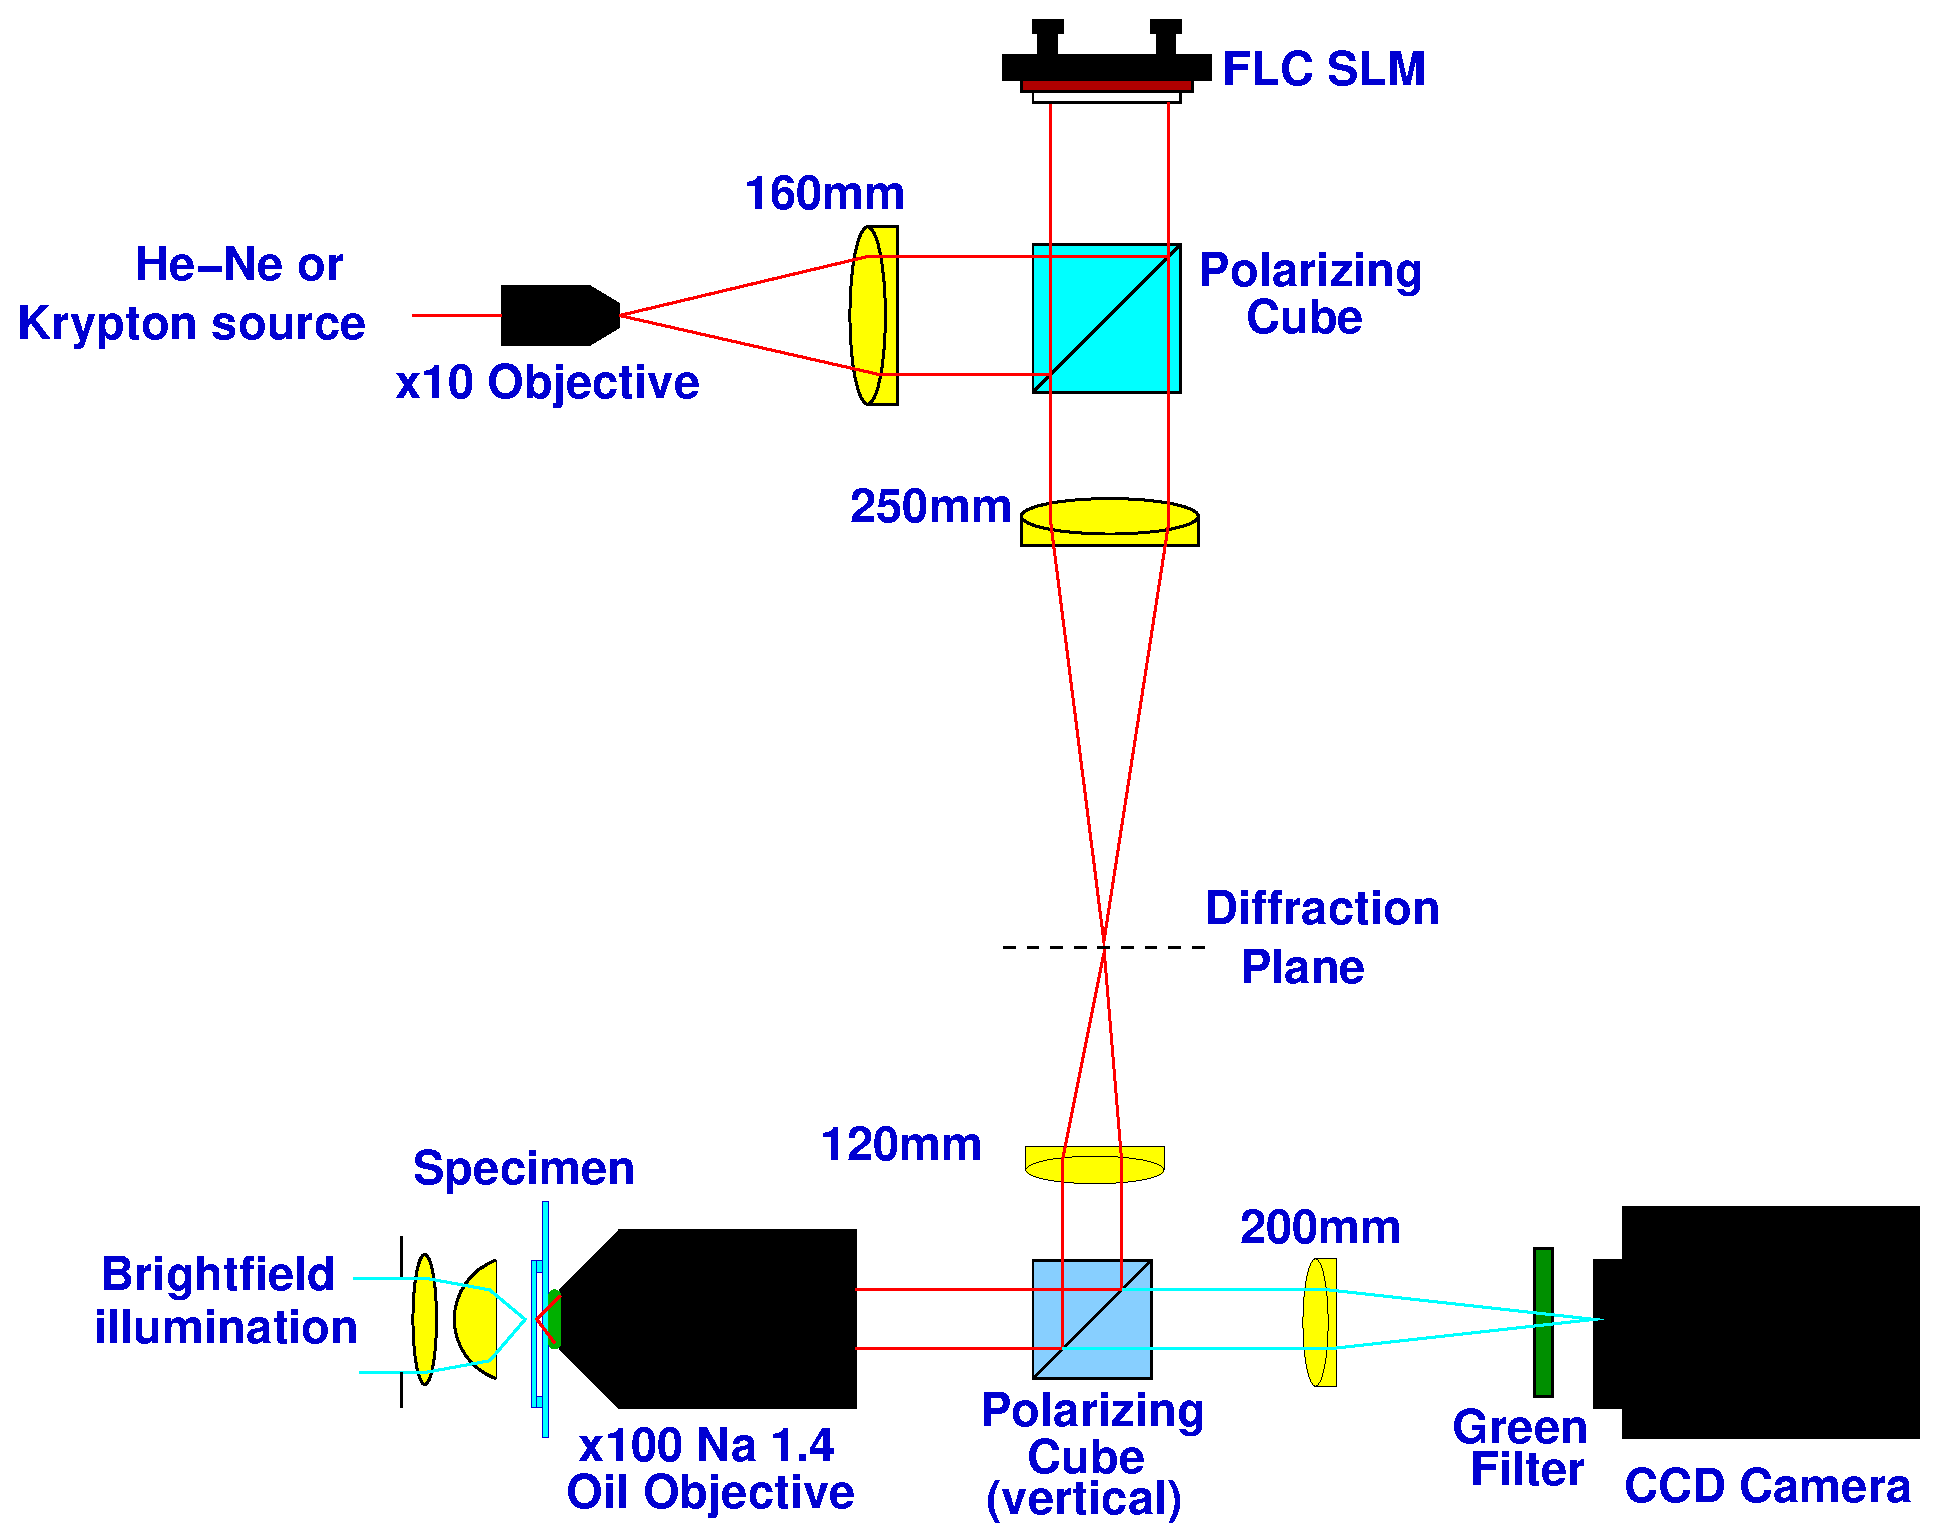
\includegraphics[width=100mm]{OpticalSystem}
% \end{center}
% \caption{Here is the optical system from the same paper
%   as the reference drawn in {\tt xfig} and include to
%   shown how such a figure in included.}
% \label{fig:prism}                 % Reference label to the figure.
% \end{figure}

At this stage it is {\em not} expected that this will be a fully-developed
research proposal, but is your chance to show what you have extracted from the
literature and how you see your own work will fit in. This section is
not expected to exceed 2 pages.
 
\section{Summary}

As short section highlighting the key aspect of your proposal.
At this stage this may be a bit uncertain and will be subject
to charge as the work progresses.
%            Now build the reference list

% \section{Risk Assessment}

\bibliographystyle{unsrt}                      % The reference style
%                This is plain and unsorted, so in the order
%                they appear in the document.


\bibliography{frb,pulsar}       % Multiple bib files.

\end{document}

